\documentclass{article}
\usepackage[utf8]{inputenc}
\usepackage{graphicx}

\title{Final Exam -- Calculus 101}
\author{Professor Ketz}
\date{March 28, 2017}

\begin{document}

\maketitle

\section{Definitions}
	\begin{itemize}
	\item{limit}
	\item{derivative}
	\item{derived function}
	\item{continuous}
	\item{integrable}
	\end{itemize}

\section{Calculations}
Evaluate the following limits
	\begin{enumerate}
	\item{ \[\lim_{x\to\infty} 100\] }
	\item{ \[\lim_{x\to\infty} \frac{3x^5 + 17x^4 - 18}{x^5 - 12x^2}\] }
	\item{ \[\lim_{h\to0}\frac{\sqrt{2(x+h)-1}-\sqrt{2x-1}}{h}\] }
	\end{enumerate}
Evaluate the following integrals
	\begin{enumerate}
	\item{ \[ \int_{0}^{10} x^2 \] }
	\item{ \[ \int_{-5}^{1} \sqrt{x} \] }
	\end{enumerate}

\section{Some fun!}
Now comes the time to see if you actually ever paid attention in this class, or if you slept through the entire semester and only showed up to the final just to pass.

\begin{center}
Who am I?
\end{center}
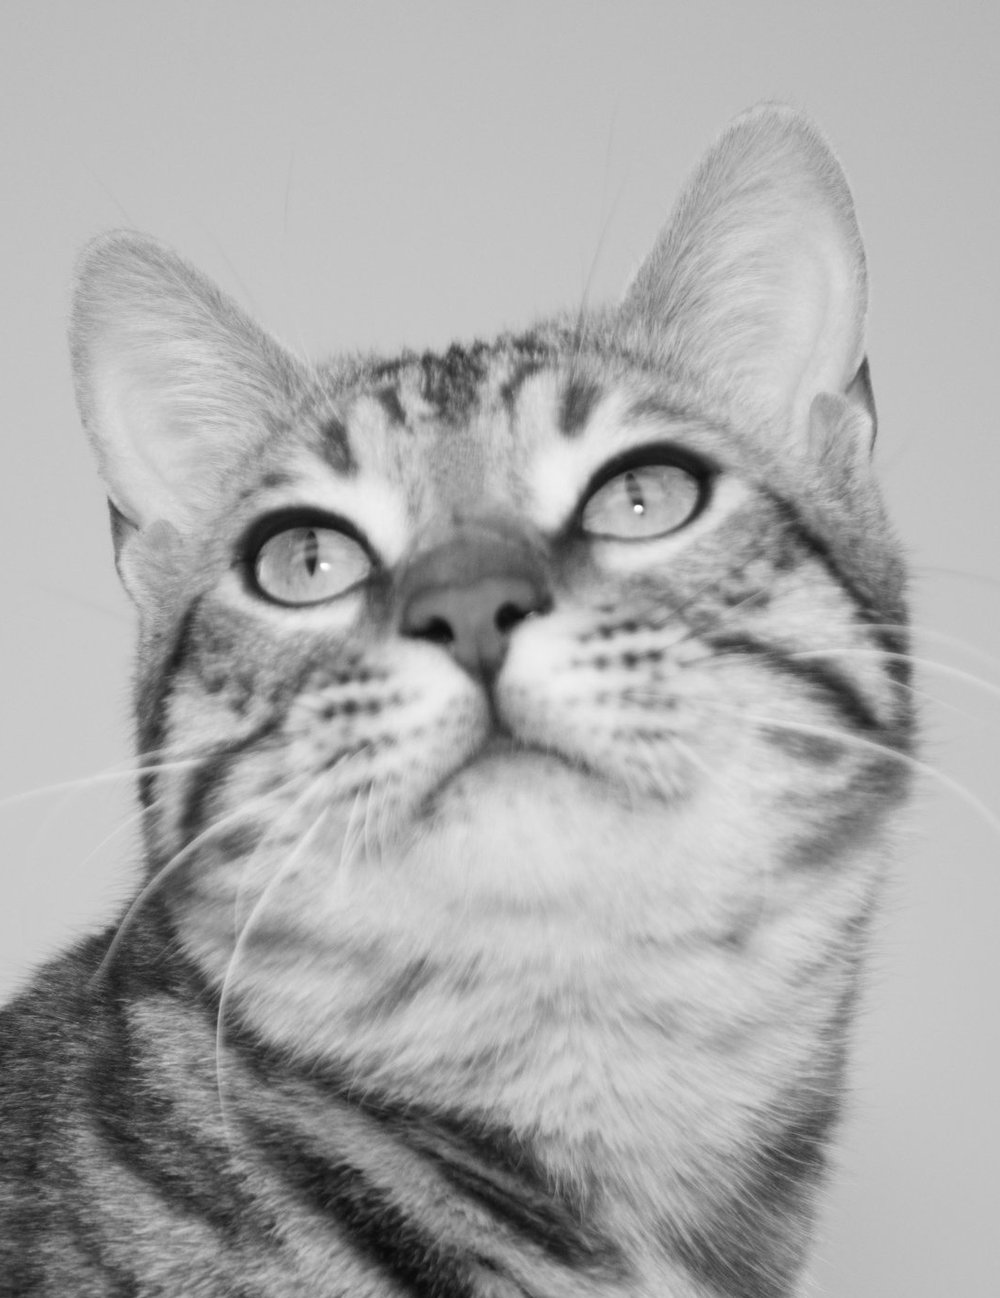
\includegraphics[width=100px]{cat.jpg}

\includegraphics[width=100px]{cat2.jpg}
\includegraphics[width=100px]{kats.jpg}
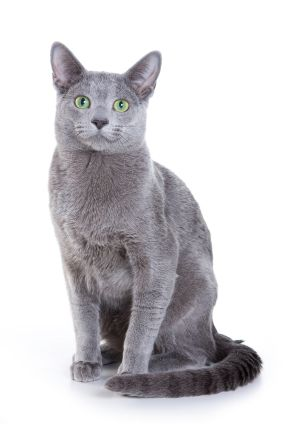
\includegraphics[width=100px]{cat3.jpg}
\end{document}
